% -*- TeX -*- -*- UK -*-
% ----------------------------------------------------------------
% arXiv Paper ************************************************
%
% Subhaneil Lahiri's template
%
% Before submitting:
%    Comment out hyperref
%    Comment out showkeys
%    Replace \input{?.tex} with its contents
%       or include ?.tex in zip/tar file
%    Put this file, the .bbl file, any picture or
%       other additional files and natbib.sty
%       file in a zip/tar file
%
% **** -----------------------------------------------------------
\documentclass[12pt]{article}
%Preamble:
\usepackage{a4wide}
\input{sl_preamble.tex}
%
% >> Only for drafts! <<
\usepackage[notref,notcite]{showkeys}
%
\input{sl_graphics_preamble.tex}
\graphicspath{{Figures/}}
%
% ----------------------------------------------------------------
%\numberwithin{equation}{section}
%\renewcommand{\baselinestretch}{1.5}
% ----------------------------------------------------------------
% New commands etc.
\input{sl_definitions.tex}
\input{sl_symbols.tex}
%matrices
%vec of ones
\newcommand{\onev}{\mathbf{e}}
%mat of ones
\newcommand{\onem}{\mathbf{E}}
%Markov matrix
\newcommand{\MM}{\mathbf{Q}}
%prob distribution
\newcommand{\pr}{\mathbf{p}}
%equilibrium distribution
\newcommand{\eq}{\pr^\infty}
%first passage times
\newcommand{\fpt}{\mathbf{T}}
%off-diag first passage times
\newcommand{\fptb}{\overline{\fpt}}
%fundamental matrix
\newcommand{\fund}{\mathbf{Z}}
%other symbols
\newcommand{\Pb}{\mathbf{P}}
\newcommand{\D}{\mathbf{D}}
\newcommand{\pib}{\boldsymbol{\pi}}
\newcommand{\Lb}{\boldsymbol{\Lambda}}
\newcommand{\etw}{\boldsymbol{\eta}^w}
\newcommand{\thb}{\boldsymbol{\theta}}
%synapse models
\newcommand{\w}{\mathbf{w}}
\newcommand{\W}{\mathbf{W}}
\newcommand{\M}{\mathbf{M}}
\newcommand{\enc}{\mathbf{K}}
\newcommand{\frg}{\W^{\mathrm{F}}}
\newcommand{\F}{\boldsymbol{\Phi}}
%superscripts
\newcommand{\pot}{^{\text{pot}}}
\newcommand{\dep}{^{\text{dep}}}
\newcommand{\potdep}{^{\text{pot/dep}}}
%with activity indep processes
\renewcommand{\hom}{\mathbf{H}}
\newcommand{\Mh}{\widetilde{\M}}
\newcommand{\frgh}{\widetilde{\W}^{\mathrm{F}}}
\newcommand{\ench}{\widetilde{\enc}}
%eigenvectors
\newcommand{\evr}{\mathbf{u}}
\newcommand{\evl}{\boldsymbol{\eta}}
%snr curves etc
\newcommand{\syn}{\vec{w}}
\newcommand{\synid}{\syn_\text{id}}
\DeclareMathOperator{\SNR}{SNR}
\DeclareMathOperator{\snr}{SNR}
\DeclareMathOperator{\NNR}{NNR}
\DeclareMathOperator{\nnr}{NNR}
\newcommand{\snrb}{\overline{\snr}}
\DeclareMathOperator{\env}{Env}
\newcommand{\rh}{\hat{r}}
\newcommand{\CA}{\mathcal{A}}
\newcommand{\CB}{\mathcal{B}}
%avoid double superscripts
\renewcommand{\pdiff}[2]{\frac{\partial #1}{\partial #2}}

% ----------------------------------------------------------------
\input{sl_theorems_preamble.tex}
% ----------------------------------------------------------------
%
%%%%%%%%%%%%%%%%%%%%%%%%%%%%%%%%%%%%%%%%%%%%%%%%%%%%%%%%%%%%%%%%%%%%%%%%%%
% Title info:
\title{Laplacian envelope}
%
% Author List:
%
\author{Subhaneil Lahiri
%
}

\begin{document}

\maketitle


%%%%%%%%%%%%%%%%%%%%%%%%%%%%%%%%%%%%%%%%%%%%%%%%%%%%%%%%%%%%%%%%%%%%%%%%%%


\begin{abstract}
  We try to find the continuous time Markov process that has the maximal Laplace transformed signal-to-noise curve.
\end{abstract}

\tableofcontents

\listoffigures

%%%%%%%%%%%%%%%%%%%%%%%%%%%%%%%%%%%%%%%%%%%%%%%%%%%%%%%%%%%%%%%%%%%%%%%%%%
% Beginning of Article:
%%%%%%%%%%%%%%%%%%%%%%%%%%%%%%%%%%%%%%%%%%%%%%%%%%%%%%%%%%%%%%%%%%%%%%%%%%

\section{Framework}\label{sec:framework}

\subsection{Recognition memory}\label{sec:recog}


We will be trying to store patterns in a set od $N$ synaptic weights, $\syn$.
Every time we try to store a pattern, these synapses are subjected to a plasticity event where each synapse is either potentiated or depressed, depending on the pattern.
we will assume that these patterns are spatially and temporally independent.

At some time, suppose we wish to determine if a given pattern is one of those that we previously attempted to store.
We wish to answer this question by looking at the synaptic weights directly (ideal observer).
For that given pattern there will be an ideal set of synaptic weights, $\synid$, where those synapses that were supposed to be potentiated are maximised and those that were supposed to be depressed are minimised.
Suppose that the given pattern was actually seen at time 0 and we are observing the synapses at time $t$.
The actual set of synaptic weights we see, $\syn(t)$, will be a vector of random variables that differs from $\synid$ due to the stochasticity of the pattern encoding and all of the other (uncorrelated) pattern that are stored after it.
As $t\to\infty$, the synaptic weights will become independent of the patter stored at $t=0$.
Thus, the vector of random variables $\syn(\infty)$ also describes the synaptic weights under the null hypothesis -- if that given pattern had never been stored.

We can test if the pattern had been previously stored by computing $\synid\cdt\syn$ and comparing it to some threshold.
For large $N$, this quantity will have a Gausssian distribution.
There will be a ROC curve as a function of this threshold:
%
\begin{equation}\label{eq:ROC}
  \begin{aligned}
  \operatorname{TPR} &= \Phi_c \prn{ \frac{ \Phi_c\inv(\operatorname{FPR}) - \snr }{ \NNR } },
  \quad\text{where } &
    \Phi_c(x) &= \int_x^\infty \frac{ \e^{-\frac{z^2}{2}} }{ \sqrt{2\pi} }\, \dz, \\&&
    \snr &= \frac{ \av{\synid\cdt\syn(t)} - \av{\synid\cdt\syn(\infty)} }{ \sqrt{\var(\synid\cdt\syn(\infty))}}, \\&&
    \NNR &= \sqrt{\frac{ \var(\synid\cdt\syn(t)) }{ \var(\synid\cdt\syn(\infty)) }},
  \end{aligned}
\end{equation}
%
and TPR/FPR are the true/false positive rates.
When the signal-to-noise ratio, $\snr$ is larger than $\Phi_c\inv(\operatorname{FPR})$, it is beneficial to decrease the noise-to-noise ratio, NNR.
In the other case, it is beneficial to increase it.
The expectations and variances are over the probability distribution of the synaptic states given the sequence of plasticity events, the probability distribution of the sequence of plasticity events themselves and the probability distribution of the pattern we are testing, $\synid$.

There are other measures of memory one could consider, \eg asymptotic error exponents.
For the Neyman-Pearson approach to hypothesis testing, the error exponent is the KL divergence:
%
\begin{equation*}
  D_\text{KL}\prn{P_0 \middle\Vert P_1} = \ln\nnr + \frac{1 + \snr^2}{2\nnr^2} - \frac{1}{2}.
\end{equation*}
%
For Bayesian hypothesis testing, the error exponent is the Chernoff distance:
%
\begin{equation*}
  D^*\prn{P_0 \middle\Vert P_1} = \max_\alpha \brc{
    \frac{1}{2} \ln\brk{\frac{1 + \alpha(\nnr^2-1)}{\nnr^{2\alpha}}} + \frac{\alpha(1-\alpha)\snr^2}{2[1 + \alpha(\nnr^2-1)]}
  }.
\end{equation*}
%

The formulae above assumed that we know the time between storage and recognition.
We should also compute the expectations and variances over probability distribution of the recall time, $t$, as well.
If we only know average time, $\tau$, a natural choice for this distribution is
%
\begin{equation}\label{eq:recogtime}
  P(t\vert\tau) = \frac{\e^{-t/\tau}}{\tau}.
\end{equation}
%
Different parts of the brain, that store memories for different timescales, could be characterised by different values of $\tau$.


\subsection{Signal-to-noise ratio}\label{sec:snr}

We will model the synapses as having two possible synaptic weights.
As we are looking at the information contained in the synaptic weights, rather than modelling the readout via electrical activity of the neurons, what values the synaptic weights actually take is irrelevant.
It will be convenient to call these two values $\pm1$.


As discussed in \autoref{sec:recog}, the signal-to-noise ratio is given by
%
\begin{equation}\label{eq:SNRdef}
  \snr(t) = \frac{\av{\syn_\text{ideal}\cdt\syn(t)} - \av{\syn_\text{ideal}\cdt\syn(\infty)}}
     {\sqrt{\var(\syn_\text{ideal}\cdt\syn(\infty))}},
\end{equation}
%
Where the averages and variances are over the probability distribution of the synaptic states given the sequence of plasticity events, the probability distribution of the sequence of plasticity events themselves and the probability distribution of the pattern we are testing, $\synid$.
If we also average over the time between storage and recognition, we have
%
\begin{equation}\label{eq:snrb}
  \snrb(\tau) = \intd[_0^\infty]{t} P(t\vert\tau) \snr(t)
   = \frac{1}{\tau} \intd[_0^\infty]{t} \e^{-t/\tau} \snr(t),
\end{equation}
%
This is similar to the average SNR up to time $\tau$, but with the hard cut-off replaced with a smooth exponential.
This can be expressed in terms of he Laplace transform of the SNR curve in \eqref{eq:SNRdef}:
%
\begin{equation}\label{eq:laplacedef}
  A(s) = \intd[_0^\infty]{t} \e^{-st} \snr(t),
  \qquad
  \snrb(\tau) = \frac{A(1/\tau)}{\tau}.
\end{equation}
%


First, let's look at the variances, remembering that the states and plasticity events of each synapse are independent and identically distributed:
%
\begin{equation}\label{eq:noise}
\begin{aligned}
  \var(\synid\cdt\syn(t))
    &= \sum_{\alpha\beta} \av{\synid^\alpha \syn^\alpha(t) \synid^\beta \syn^\beta(t)}
    - \Big(\sum_{\alpha} \av{\synid^\alpha \syn^\alpha(t)} \Big)^2 \\
    &= \sum_{\alpha} \av{(\synid^\alpha)^2(\syn^\alpha(t))^2}
    + \sum_{\alpha\neq\beta} \av{\synid^\alpha\syn^\alpha(t)}\av{\smash{\synid^\beta}\smash{\syn^\beta}(t)}
    %\\&\phantom{= \sum_{\alpha}  \av{(\synid^\alpha)^2(\syn^\alpha(t))^2}}
    - \Big(\sum_{\alpha} \av{\synid^\alpha \syn^\alpha(t)} \Big)^2  \\
    &= N\av{1}
    + N(N-1)\av{\synid^1 \syn^1(t)}^2
    - N^2\av{\synid^1 \syn^1(t)}^2 \\
    &= N(1-\av{\synid^1 \syn^1(t)}^2),
\end{aligned}
\end{equation}
%
where we used $\syn^\alpha=\pm1$.
We can compute $\var(\syn_\text{ideal}\cdt\syn(\infty))$ by taking $t\to\infty$.

For the numerator, we can write
%
\begin{equation}\label{eq:overlapex}
  \av{\syn_\text{ideal}\cdt\syn(t)} = \sum_\alpha\av{\syn^\alpha_\text{ideal}\syn^\alpha(t)}
   = N \av{\syn^1_\text{ideal}\syn^1(t)},
\end{equation}
%
If the elements of $\synid$ take values $\pm1$ with probability $f\potdep$,
%
\begin{equation}\label{eq:overlapone}
  \av{\syn^1_\text{ideal}\syn^1(t)} = f\pot \av{\syn^1(t)}_{\text{pot},t=0} - f\dep \av{\syn^1(t)}_{\text{dep},t=0}
\end{equation}
%
To compute this quantity, we will need to discuss how we model individual synapses.




\subsection{Markov models of synapses}\label{sec:markovsynapse}

We model a synapse as having $M$ internal states.
The synaptic weight depends deterministically on the state, given by the $M$-element column vector $\w$.
We denote the probability distribution across these states by the row vector $\pr(t)$.
We denote a column vector of ones by $\onev$, so the normalisation condition is $\pr(t)\onev=1$.

When the synapse is subjected to a plasticity event the internal state will change stochastically, described by the matrices $\M\potdep$ whose $i,j$ elements are the transition probabilities from state $i$ to state $j$.
The matrices $\M\potdep$ are transition matrices of discrete time Markov processes.
Their elements must satisfy the following constraints
%
\begin{equation}\label{eq:constr}
\begin{aligned}
  \M\potdep_{ij} &\geq 0, &\qquad
  \sum_j \M\potdep_{ij} &= 1.
\end{aligned}
\end{equation}
%
The upper bounds $\M\potdep_{ij} \leq 1$ follow automatically from these.

If we treat the off diagonal elements as the independent degrees of freedom, with the off diagonal elements determined by the row sum constraints (second column of \eqref{eq:constr}), the constraints are
%
\begin{equation}\label{eq:constri}
  \M\potdep_{i \neq j} \geq 0, \qquad
  \sum_{j\neq i} \M\potdep_{ij} \leq 1.
\end{equation}
%
The second of these will be referred to as the ``diagonal'' constraint.

Given a sequence of plasticity events at times $t_1,t_2,t_3,\ldots$, the probability distribution across the internal states at time $t_n$ is
%
\begin{equation}\label{eq:plastseq}
  \pr(t_n) = \pr(t_0)  \M\pot \M\dep \M\dep \M\pot \M\dep \M\pot \M\pot \M\dep \ldots \M\pot .
\end{equation}
%
If the probability of a given plasticity event being potentiating/depressing is $f\potdep$, the probability of the sequence above (conditioned on the number of events) is given by $f\pot f\dep f\dep f\pot f\dep f\pot f\pot f\dep \ldots f\pot$.

In computing the expectation in \eqref{eq:overlapone} the plasticity event that occurs at $t=0$ is fixed, but all of the previous and subsequent events are marginalised over.
If we marginalise over the types (potentiating/depressing) of these other events (conditioned on the number of events) we find
%
\begin{multline}\label{eq:plastseqtypes}
  \pr(t_n) = \pr(t_0) (f\pot\M\pot+f\dep\M\dep)  \ldots (f\pot\M\pot+f\dep\M\dep) \\
    \M\potdep (f\pot\M\pot+f\dep\M\dep) \ldots (f\pot\M\pot+f\dep\M\dep),
\end{multline}
%
where the factor of $\M\potdep$ is the event at $t=0$.
If we expand out all of the parenthetical factors, we will get a sum of terms of the form \eqref{eq:plastseq} weighted by their probabilities.

If $t_0 \ll 0$, the effect of the large number of earlier events will be to put the synapse in the steady state distribution, $\eq$, of the stochastic process $(f\pot\M\pot+f\dep\M\dep)$:
%
\begin{equation}\label{eq:plastseqeq}
  \pr(t_n) = \eq \M\potdep (f\pot\M\pot+f\dep\M\dep)^n,
\end{equation}
%
where $n$ is the number of plasticity events that took place.

If the plasticity events occur at Poisson rate $r$, the probability of $n$ events occurring in time $t$ is given by a Poisson distribution with mean $rt$.
If we marginalise over $n$ as well
%
\begin{equation}\label{eq:plastseqav}
\begin{aligned}
  P(\text{state}=i,t \mid \text{pot/dep},0)
    &= \sum_n \frac{(rt)^n}{n!} \e^{-rt} \eq \M\potdep (f\pot\M\pot+f\dep\M\dep)^n \\
    &= \brk{ \eq \M\potdep\, \e^{rt(f\pot\M\pot+f\dep\M\dep-\I) } }_i,
\end{aligned}
\end{equation}
%
where $\eq$ is the steady state distribution of the continuous time transition matrix that appears in the exponential:
%
\begin{equation}\label{eq:eq}
  \eq\frg = 0,
  \qquad\text{where}\quad
  \frg = f\pot\M\pot + f\dep\M\dep - \I.
\end{equation}
%



This results in
%
\begin{equation}\label{eq:overlapwt}
\begin{aligned}
  \av{\syn^1_\text{ideal}\syn^1(t)} &= \eq (f\pot\M\pot-f\dep\M\dep)\, \e^{rt\frg} \w, \\
  \av{\syn^1_\text{ideal}\syn^1(\infty)} &= \eq (f\pot\M\pot-f\dep\M\dep)\, \onev\eq \w \\
         &= \eq (f\pot\onev-f\dep\onev)\, \eq \w \\
         &=  (f\pot-f\dep)\, \eq \w \\
         &=  (f\pot-f\dep)\, \eq \e^{rt\frg} \w .
\end{aligned}
\end{equation}
%
Combining these allows us to write the numerator of \eqref{eq:SNRdef} as
%
\begin{equation}\label{eq:signal}
\begin{aligned}
  \av{\syn_\text{ideal}\cdt\syn(t)} - \av{\syn_\text{ideal}\cdt\syn(\infty)}
    &= N \eq \enc \, \e^{(r\frg+\hom)t} \w , \\
    \text{where} \qquad
  \enc &= f\pot(\M\pot-\I)-f\dep(\M\dep-\I)
\end{aligned}
\end{equation}
%
Combining with \eqref{eq:noise} gives
%
\begin{equation}\label{eq:SNRcurveExact}
  \SNR(t) = \frac{\sqrt{N} \eq \enc\,\e^{rt\frg}\w}
                 {\sqrt{1-(f\pot-f\dep)^2(\eq\w)^2}}.
\end{equation}
%
%We can absorb $\hom$ into $\M\potdep$ by defining
%%
%\begin{equation}\label{eq:absorbhom}
%\begin{aligned}
%  \Mh\potdep &= \M\potdep + \frac{\hom}{2rf\potdep},
%  &\qquad
%  \frgh &= f\pot\Mh\pot + f\dep\Mh\dep - \I,
%  \\&&
%  \ench &= f\pot(\Mh\pot-\I)-f\dep(\Mh\dep-\I).
%\end{aligned}
%\end{equation}
%%
%Then the SNR curve is
%%
%\begin{equation}\label{eq:SNRcurvehom}
%  \SNR(t) = \frac{\sqrt{N}  \eq \enc \,\e^{rt\frg}\w}
%                 {\sqrt{1-(f\pot-f\dep)^2(\eq\w)^2}}.
%\end{equation}
%%
The denominator will not play any role in what follows, as the models that maximize the various measures of memory performance all have some sort of balance between potentiation and depression, either with $f\pot=f\dep$ or $\eq_+=\eq_-$.
We can perform the maximisation in two steps.
First maximise the numerator at fixed $\eq\w$.
Then maximise the ratio \wrt $\eq\w$.
This will allow us to ignore the denominator until the very end.



We can then treat the off-diagonal elements of $\M\potdep$ as the independent degrees of freedom, subject to these constraints, when maximising the SNR.
The diagonal elements are determined by setting the row sums to 1.
We then have
%
\begin{equation}\label{eq:derivpd}
  \pdiff{\M\pot_{ij}}{\M\pot_{mn}} = \pdiff{\M\dep_{ij}}{\M\dep_{mn}} = \delta_{im}(\delta_{jn}-\delta_{jm}),
  \qquad
  \pdiff{\M\pot_{ij}}{\M\dep_{mn}} = \pdiff{\M\dep_{ij}}{\M\pot_{mn}} = 0.
\end{equation}
%
It will also be convenient to define the differential operators
%
\begin{equation}\label{eq:pertfe}
  \pdiff{}{\frg_{ij}} = \frac{1}{2f\pot} \pdiff{}{\M\pot_{ij}} + \frac{1}{2f\dep} \pdiff{}{\M\dep_{ij}},
  \qquad
  \pdiff{}{\enc_{ij}} = \frac{1}{2f\pot} \pdiff{}{\M\pot_{ij}} - \frac{1}{2f\dep} \pdiff{}{\M\dep_{ij}},
\end{equation}
%
these satisfy
%
\begin{equation}\label{eq:derivfe}
  \pdiff{\frg_{ij}}{\frg_{mn}} = \pdiff{\enc_{ij}}{\enc_{mn}} = \delta_{im}(\delta_{jn}-\delta_{jm}),
  \qquad
  \pdiff{\frg_{ij}}{\enc_{mn}} = \pdiff{\enc_{ij}}{\frg_{mn}} = 0.
\end{equation}
%

If we wish to use the off-diagonal elements of $\frg$ and $\enc$ as the degrees of freedom, the constraints are
%
\begin{equation}\label{eq:constrfe}
\begin{aligned}
  \frg_{i \neq j}   &\geq \abs{ \enc_{i \neq j} }, &\qquad
  \sum_{j\neq i}\frg_{ij} \pm \abs{ \enc_{ij} } &\leq f\potdep, \\
  \sum_j \frg_{ij} &=0, &
  \sum_j \enc_{ij} &=0.
\end{aligned}
\end{equation}
%




\section{Laplace transform}\label{sec:laplace}

\subsection{Fundamental matrix \etc}\label{sec:lfund}

In analogy to the generalised fundamental matrix of a Markov chain \cite{Kemeny1981fund}, define
%
\begin{equation}\label{eq:lfund}
  \fund(s) = (s\I +\onev\pib -\MM)\inv,
\end{equation}
%
where $\pib$ is an arbitrary row vector satisfying $\pib\onev = \frac{1}{\tau_0} \neq 0$.
This reduces to the fundamental matrix at $s=0$.
We can see that $\onev$ is an eigenvector:
%
\begin{equation}\label{eq:lfundrowsum}
  \fund(s)\onev = \frac{\tau_0}{1+s\tau_0}\onev.
\end{equation}
%
Suppose we have some row vector $\mathbf{a}$ such that $\mathbf{a}\onev=0$.
Then $\mathbf{a}\fund(s)$ is independent of $\pib$:
%
\begin{equation}\label{eq:alfund}
  \pdiff{(\mathbf{a}\fund(s))_i}{\pib_k} = -(\mathbf{a}\fund(s)\onev) \fund_{ki}(s)
      = -\frac{\tau_0}{1+s\tau_0} (\mathbf{a}\onev) \fund_{ki}(s) = 0.
\end{equation}
%


Then we also define
%
\begin{equation}\label{eq:lfptb}
  \fptb(s) = (\onem\fund\dg(s)-\fund(s))\D,
  \qquad
  \fptb_{ij}(s) = \frac{\fund_{jj}(s)-\fund_{ij}(s)}{\eq_j}.
\end{equation}
%
This reduces to the first passage time matrix at $s=0$, but at other $s$ there is (probably) no relation.

Using the exact same proof as in the case $s=0$, we see that the quantity
%
\begin{equation}\label{eq:lkemeny}
  \eta(s) = \sum_j \fptb_{ij}(s)\eq_j
\end{equation}
%
is independent of the starting state $i$, but now $\eta(s) = \tr\fund(s) - \frac{\tau}{1+s\tau}$.
We can the define
%
\begin{equation}\label{eq:lpmixtime}
  \eta^{\pm}_i(s) = \sum_j \fptb_{ij}(s)\eq_j \prn{\frac{1\pm\w_j}{2}} =  \sum_{j\in\pm} \fptb_{ij}(s)\eq_j.
\end{equation}
%
We can arrange the states in order of decreasing $\eta^{+}_i(s)$ or increasing $\eta^{-}_i(s)$.
It will be more convenient to use the quantities
%
\begin{equation}\label{eq:lwpmixtime}
  \etw_i(s) = \sum_j \fptb_{ij}(s)\eq_j \w_j
    = \eta^+_i(s) - \eta^-_i(s) =2\eta^+_i(s) - \eta(s) =\eta(s) - 2\eta^-_i(s) .
\end{equation}
%
Arranging the states in order of decreasing $\etw_i(s)$ is the same as the order of decreasing $\eta^{+}_i(s)$ or increasing $\eta^{-}_i(s)$.
These quantities can still be used when $\w$ takes more than two values.



\subsection{Laplace transform of SNR curve}\label{sec:laplaceSNR}

Consider the Laplace transform of the evolution operator:
%
\begin{equation}\label{eq:levol}
  \mathbf{G}(s) = \intd[_0^{\infty}]{t} \e^{(\MM-s) t}.
\end{equation}
%
For $\Re s>0$, we have
%
\begin{equation}\label{eq:levolcalc}
  (s-\MM)\mathbf{G}(s) = \intd[_0^{\infty}]{t} (s-\MM)\e^{(\MM-s) t} = \brk{-\e^{(\MM-s) t}}_0^{\infty} = \I.
\end{equation}
%
As $(s-\MM)$ is invertible for $\Re s>0$, because the real part of all eigenvalues of $\MM$ are nonpositive, we have
%
\begin{equation}\label{eq:levolres}
  \mathbf{G}(s) = (s-\MM)\inv.
\end{equation}
%
For $s=0$, we can avoid problems by replacing $\mathbf{G}(s) \to \fund(s)$.

Now consider the Laplace transform of the SNR curve \eqref{eq:SNRcurveExact} (ignoring the denominator)
%
\begin{equation}\label{eq:lsnr}
\begin{aligned}
  A(s) &= \intd[_0^{\infty}]{t} \e^{-st}\SNR(t) \\
   &= \intd[_0^{\infty}]{t} \frac{ \sqrt{N} \eq \enc \e^{(r\frg-s)t} \w }{ \sqrt{1-(f\pot-f\dep)^2(\eq\w)^2} } \\
   &= \frac{\sqrt{N} \eq \enc \prn{s - r\frg}\inv \w }{\sqrt{1-(f\pot-f\dep)^2(\eq\w)^2}}.
\end{aligned}
\end{equation}
%
This expression is ill-behaved at $s=0$.
Thanks to \eqref{eq:alfund}, we can solve this by the replacement $\mathbf{G}(s) \to \fund(s)$, as $\enc\onev=0$.
%
\begin{equation}\label{eq:larea}
\begin{aligned}
  \hat{A}(s) = A(s) \sqrt{\frac{{{1-(f\pot-f\dep)^2(\eq\w)^2}}}{N}}  &=  \eq \enc \fund(s) \w \\
    &= \sum_{ijk} \eq_i \enc_{ij} \prn{\fptb_{ik}(s)-\fptb_{jk}(s)} \eq_k \w_k \\
    &= \sum_{ij}  \eq_i \enc_{ij} (\etw_{i}(s) - \etw_{j}(s)).
\end{aligned}
\end{equation}
%
Note that $A(0)=A$, the area, and $\lim_{s\to\infty} \brc{sA(s)} = \SNR(0)$, the initial SNR.

In analogy with the case $s=0$, we define
%
\begin{equation}\label{eq:lareacoeffs}
  \begin{aligned}
    c_k(s) &= \sum_{ij} \eq_i \enc_{ij} \prn{\fptb_{ik}(s)-\fptb_{jk}(s)}, \\
    a_j(s) &= \sum_{jk} \eq_j \enc_{jk} (\etw_{j}(s) - \etw_{k}(s)), \\
    \thb_i(s) &= \sum_j \fptb_{ij}(0)\ a_j(s), \\
  \end{aligned}
    \implies
    \hat{A}(s) = \sum_k c_k(s) \eq_k \w_k
      = \sum_i a_i(s).
\end{equation}
%

\subsection{Derivatives}\label{sec:lderiv}

Using the same approach as the area bound in \cite{Lahiri2013synapse} we find that the derivatives are
%
\begin{equation}\label{eq:lAdiff}
  \pdiff{\hat{A}(s)}{\M\potdep_{mn}}
     = f\potdep \eq_m \prn{ r \brk{\thb_m(s) - \thb_n(s)}
     +\prn{rc_m(s) \pm 1} \brk{\etw_m(s) - \etw_n(s)} },
\end{equation}
%
with the upper/lower sign in $\pm$ corresponding to derivatives \wrt $\M\potdep$.
The term with $\Theta(s)$ comes from differentiating $\eq$, the term with $c(s)$ comes from differentiating $\etw(s)$ and the term with $\pm1$ comes from differentiating $\enc$ in \eqref{eq:larea}.

To write down the Hessian, we will first define some notation.
We define the matrix $\mathbf{X}(s) = \fund(0) \enc \fund(s)$.
Given a four-index array $H_{ijkl}$, we define $H\trans_{ijkl} = H_{klij}$.
Then we denote
%
\begin{equation}\label{eq:hessparts}
\begin{aligned}
  R_{ijkl} &=
    &&\eq_i \brc{\fund_{ik}(0) - \fund_{jk}(0)} \brc{\thb_k(s) - \thb_l(s)} \\
    &&&+ \eq_i \brc{\mathbf{X}_{ik}(s) - \mathbf{X}_{jk}(s)} \brc{\etw_k(s) - \etw_l(s)} \\
    &&&+ \eq_i c_i(s) \brc{\fund_{ik}(s) - \fund_{jk}(s)} \brc{\etw_k(s) - \etw_l(s)},  \\
  S_{ijkl} &=
    &&\eq_i \brc{\fund_{ik}(0) - \fund_{jk}(0)} \brc{\etw_k(s) - \etw_l(s)} \\
    &&&+ \eq_k \brc{\fund_{ki}(s) - \fund_{li}(s)} \brc{\etw_i(s) - \etw_j(s)}.
\end{aligned}
\end{equation}
%
Then we can write the Hessian as
%
\begin{equation}\label{eq:hessian}
\begin{aligned}
  \pdiff{^2\hat{A}(s)}{\M\pot_{ij} \partial\M\pot_{kl}} &=
     (f\pot)^2   [R + R\trans + S + S\trans]_{ijkl}, \\
  \pdiff{^2\hat{A}(s)}{\M\pot_{ij} \partial\M\dep_{kl}} &=
     f\pot f\dep [R + R\trans - S + S\trans]_{ijkl}, \\
  \pdiff{^2\hat{A}(s)}{\M\dep_{ij} \partial\M\pot_{kl}} &=
     f\pot f\dep [R + R\trans + S - S\trans]_{ijkl}, \\
  \pdiff{^2\hat{A}(s)}{\M\dep_{ij} \partial\M\dep_{kl}} &=
     (f\dep)^2   [R + R\trans - S - S\trans]_{ijkl}, \\
\end{aligned}
\end{equation}
%
This is useful in numerical maximisation.

\section{Upper bounds}\label{sec:upperbnds}



\subsection{Initial SNR}\label{sec:initial}

The initial SNR is:
%
\begin{equation}\label{eq:initdef}
  \snr(0) = \snrb(0) = \lim_{s\to\infty} sA(s).
\end{equation}
%

As shown in \cite{Lahiri2013synapse}, this satisfies the inequality
%
\begin{equation}\label{eq:initbnd}
  \snr(0) \leq \sqrt{N},
\end{equation}
%
The model that saturates this bound is (equivalent to) a two-state model with deterministic transitions and $f\potdep=\frac{1}{2}$.

\subsection{Area bound}\label{sec:area}

The area under the SNR curve is:
%
\begin{equation}\label{eq:areadef}
  \intd[_0^\infty]{t} \snr(t) = \lim_{\tau\to\infty} \tau \snrb(\tau) = A(0).
\end{equation}
%

As shown in \cite{Lahiri2013synapse}, this satisfies the inequality
%
\begin{equation}\label{eq:areabnd}
  A(0) \leq \frac{\sqrt{N}(M-1)}{r}.
\end{equation}
%
The model that saturates this bound is one of serial topology with $\eq$ concentrated symmetrically at the two end states.



\subsection{Envelope}\label{sec:envelope}

Now we introduce an eigenvector decomposition for $-\frg$:
%
\begin{equation}\label{eq:eigendecomp}
  \frg = - \sum_a q_a \evr^a \evl^a,
  \quad
  \evl^a \evr^b = \delta_{ab},
  \quad
  \frg \evr^a = -q_a \evr^a,
  \quad
  \evl^a \frg = -q_a \evl^a.
\end{equation}
%
Then we can write
%
\begin{equation}\label{eqsnreig}
  \snr(t) = \sqrt{N}\sum_a \CI_a \e^{-rt/\tau_a},
  \qquad
  \snrb(\tau) = \sqrt{N}\sum_a \frac{\CI_a}{1+r\tau/\tau_a},
\end{equation}
%
where
%
\begin{equation}\label{eq:snrcoeffs}
  \CI_a = (\eq \ench \evr^a) (\evl^a \w),
  \qquad
  \tau_a = \frac{1}{q_a}.
\end{equation}
%
From \eqref{eq:areabnd} and \eqref{eq:initbnd}, we see that they are subject to the constraints
%
\begin{equation}\label{eq:coeffconstr}
  \sum_a \CI_a \tau_a \leq M-1,
  \qquad
  \sum_a \CI_a \leq 1.
\end{equation}
%
No doubt there are many other constraints that these quantities must satisfy, but we can see what these ones imply for the $\snrb(\tau)$ by maximising it subject to these constraints.

Consider the Lagrangian
%
\begin{equation}\label{eq:envlagrangian}
  \CL = \sum_a \frac{\CI_a}{1+r\tau/\tau_a} + \mu_\CI \prn{1 - \sum_a \CI_a} + \mu_\CA \prn{(M-1) - \sum_a \CI_a \tau_a}.
\end{equation}
%
The Karush-Kuhn-Tucker necessary conditions for a maximum are
%
\begin{equation}\label{eq:envKTcond}
  \pdiff{\CL}{\CI_a} = 0, \qquad
  \pdiff{\CL}{\tau_a} = 0, \qquad
  \mu_\alpha \geq 0, \qquad
  \pdiff{\CL}{\mu_\alpha} \geq 0, \qquad
  \mu_\alpha\pdiff{\CL}{\mu_\alpha} = 0.
\end{equation}
%
These are solved by
%
\begin{equation}\label{eq:envsol}
\begin{gathered}
  \CI_1 = 1, \qquad
  \CI_{a>1} = 0, \qquad
  \tau_1 = M-1, \\
  \mu_\CI = \frac{(M-1)^2}{(r\tau + (M-1))^2}, \qquad
  \mu_\CA = \frac{r\tau}{(r\tau+(M-1))^2}. \qquad
\end{gathered}
\end{equation}
%
This leads to the envelope
%
\begin{equation}\label{eq:env}
  \snrb(\tau) \leq \frac{\sqrt{N}(M-1)}{r\tau + (M-1)}.
\end{equation}
%
This is the envelope (``memory frontier'') that we can prove.
Finding more constraints would lower it.
Clearly there have to be more constraints, as \eqref{eq:envsol} indicates that this would be achieved by the same model at all times.
This model would have to saturate both the initial SNR bound \eqref{eq:initbnd} and the area bound \eqref{eq:areabnd}, whereas we saw that they were achieved by different models, which perform well at short/long timescales respectively.

This envelope is shown in \autoref{fig:envproven}.


\begin{figure}[tb]
  \centering
  % Requires \usepackage{graphicx}
  \includegraphics[width=0.8\linewidth]{LenvProven.eps}
  \caption[Proven envelope]{The memory curve envelope that we can prove, \eqref{eq:env}.
  The number of synapses $N=10^4$ and the number of states $M=12$.
  The dashed lines indicate the initial SNR bound, \eqref{eq:initbnd}, and the area bound, \eqref{eq:areabnd}, from \cite{Lahiri2013synapse}.}\label{fig:envproven}
\end{figure}




\section{Finite time}\label{sec:finite}

Now we'll maximise $\snrb(\tau)$ for some fixed $\tau$, subject to the constraints \eqref{eq:constr}.
First, we will maximise the numerator of \eqref{eq:lsnr} holding $\eq\w$ fixed.
We can maximise the ration \wrt $\eq\w$ later.
Consider the Lagrangian
%
\begin{equation}\label{eq:finitelagrangian}
\begin{aligned}
  \CL =&\, \sum_{ij} \eq_i \enc_{ij} (\etw_i(s) - \etw_j(s))
        +\sum_{i j} \prn{ f\pot\mu\pot_{ij} \M\pot_{ij} + f\dep\mu\dep_{ij} \M\dep_{ij} }\\
        &+ \lambda \prn{ \Delta\pr - \sum_i \eq_i\w_i },
\end{aligned}
\end{equation}
%
where $\Delta\pr$ is the constant value we are holding $\eq\w$ at.
After maximising
The Karush-Kuhn-Tucker necessary conditions for a maximum are
%
\begin{equation}\label{eq:KTfinite}
  \pdiff{\CL}{\M\potdep_{ij}} = 0, \quad
  \mu\potdep_{ij} \geq 0, \quad
  \pdiff{\CL}{\mu\potdep_{ij}} \geq 0, \quad
  \mu\potdep_{ij}\pdiff{\CL}{\mu\potdep_{ij}} = 0, \quad
  \pdiff{\CL}{\lambda} = 0.
\end{equation}
%
The derivatives, for $m \neq n$ are
%
\begin{equation}\label{eq:finitederivs}
\begin{aligned}
  \frac{1}{f\potdep} \pdiff{\CL}{\Mh\potdep_{mn}} =& \,
      \eq_m \prn{ r \brk{\thb_m(s) - \thb_n(s)}
     +\prn{rc_m(s) \pm 1} \brk{\etw_m(s) - \etw_n(s)} } \\
     &+ \mu\potdep_{mn} -  \mu\potdep_{mm}
     + \lambda \eq_m \sum_i (\fptb_{mi}(0)-\fptb_{ni}(0)) \eq_i\w_i.
\end{aligned}
\end{equation}
%
These have the same form as for $s=0$, which allowed us to argue that the model with maximal area must have the serial topology, \cite{Leibold2008serial,Ben-DayanRubin2007sparse}.

The one missing ingredient is the scale invariance.
Define the scale transformation:
%
\begin{equation}\label{eq:scale}
  \lambda * \M = (1-\lambda)\I + \lambda \M.
\end{equation}
%
The Laplace transform has the following scaling property
%
\begin{equation}\label{eqlaplacescale}
  A(\lambda s;\lambda * \M\potdep) = A(s;\M\potdep).
\end{equation}
%
At $s=0$, it is scale invariant.
This means that we can take a pair of matrices that violates the ``diagonal'' constraints (second inequality of \eqref{eq:constri}) and use the scale transform \eqref{eq:scale} to construct a pair of matrices that satisfy the ``diagonal'' constraints and have the same area.
This allowed us to ignore the diagonal constraints.
We can't do that for $s>0$.

However, we do have numerical evidence that the model that maximises the Laplace transform does have the serial topology.
In \autoref{fig:envnum} we see the result of numerical maximisation of \eqref{eq:finitelagrangian}.
We see that restricting to the serial topology does not make the performance any worse.
In fact, it slightly improves the performance, but this can be ascribed to the numerical optimisation problem being easier.
Assuming that the optimiser did find the global maximum, this provides evidence for our conjecture  that the model that maximises the Laplace transform must have the serial topology.


\begin{figure}[tb]
  \centering
  % Requires \usepackage{graphicx}
  \includegraphics[width=0.8\linewidth]{LenvNum.eps}\\
  \caption[Numerical envelope]{Numerical envelope for the memory curve, \eqref{eq:snrb}, when $f\potdep=\frac{1}{2}$, the number of synapses $N=10^4$ and the number of states $M=12$.
  The dashed red line indicates maximisation of the memory curve over the space of all matrices satisfying the constraints \eqref{eq:constr}.
  The solid red line indicates maximisation over models with the serial topology, \ie potentiation only moves up one state and depression only moves down one state.
  The solid grren line indicates the proven envelope, \eqref{eq:env}.}\label{fig:envnum}
\end{figure}

\begin{figure}[tbp]
  \centering
  % Requires \usepackage{graphicx}
  \begin{myenuma}
  \item\aligntop{\includegraphics[width=0.45\linewidth]{Lenv07.eps}}
  \item\aligntop{\includegraphics[width=0.45\linewidth]{Lenv13.eps}}
  \item\aligntop{\includegraphics[width=0.45\linewidth]{Lenv21.eps}}
  \item\aligntop{\includegraphics[width=0.45\linewidth]{Lenv27.eps}}
  \item\aligntop{\includegraphics[width=0.45\linewidth]{Lenv36.eps}}
  \item\aligntop{\includegraphics[width=0.45\linewidth]{Lenv51.eps}}
  \end{myenuma}
  \caption[Optimal models]{The models that constitute the numeric envelope in \autoref{fig:envnum}.
  The plot to the left of each frame indicates the memory curve of the model shown to the right in blue, with the numeric envelope for models with the serial topology in red and the proven envelope, \eqref{eq:env}, in green.
  The bar graph in the upper right of each frame indicates the transition probabilities from the state to the left of each bar to the state on its right, under potentiation.
  The bar graph in the lower right of each frame indicates the transition probabilities from the state to the right of each bar to the state on its left, under depression.
  The heat map in the centre right of each frame indicates the equilibrium probability distribution for each state.
  See the video for the full set of models.}\label{fig:envvid}
\end{figure}



\section{Nearly uniform serial models}\label{sec:serial}

\begin{figure}[tb]
  \centering
  % Requires \usepackage{graphicx}
  \begin{myenuma}
    \item\aligntop{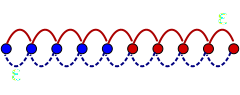
\includegraphics[width=0.26\linewidth]{serial_n.svg}}\hspace{0.02\linewidth}\label{fig:serial_uniform}
    \item\aligntop{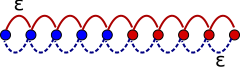
\includegraphics[width=0.26\linewidth]{serial_sticky.svg}}\hspace{0.02\linewidth}\label{fig:serial_sticky}
    \item\aligntop{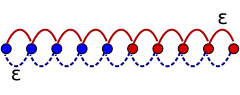
\includegraphics[width=0.26\linewidth]{serial_shorten.svg}}\label{fig:serial_shorten}
  \end{myenuma}
  \caption[Heuristic optimal models]{Heuristics for models that maximise memory curve.
  All unlabelled arrowshave transition probabilities equal to 1.
  At one particular time, the model is (\ref{fig:serial_uniform}) the uniform serial model with $M$ states.
  At later times, the model has (\ref{fig:serial_sticky}) ``sticky'' end states with low exit transition probabilities, tending to the area maximising model.
  At earlier times, the model is (\ref{fig:serial_shorten}) progressively shortened by reducing the transition probability to the end states.
  Once this reaches zero, we discard the old end state and work on the new end state.} \label{fig:heuristicmodels}
\end{figure}


Looking at them models that were found by numerical maximisation in \autoref{fig:envvid} (see the video for the full set of models), suggests we look at the particular set of models, shown in \autoref{fig:heuristicmodels}.

At one particular time, the model is (\ref{fig:serial_uniform}) the uniform serial model with $M$ states.
At later times, the model has (\ref{fig:serial_sticky}) ``sticky'' end states with low exit transition probabilities, tending to the area maximising model as $\tau\to\infty$.
At earlier times, the model is (\ref{fig:serial_shorten}) progressively shortened by reducing the transition probability to the end states.
Once this reaches zero, we discard the old end state and shorten further by reducing the transition probability to the new end state (as one can see from \autoref{fig:envvid} and the video, this is not quite true, but it is close enough to true to get a reasonable approximation to the envelope).
Once the length has been reduced to $M=2$, the model is not shortened any further and the two-state model with deterministic transitions maximises the memory curve for all earlier times.

These models' Laplace transforms can be computed analytically, as we will see below, leading to a heuristic envelope.
All of these calculations will be performed at $f\potdep=\frac{1}{2}$, so the denominator will play no role.
We will work in units such that $r=1$ temporarily, only restoring $r$ at the end.


\subsection{Uniform serial model}\label{sec:serial_uniform}


Here we will look at the model in \autoref{fig:heuristicmodels}\ref{fig:serial_uniform}.
Looking at \eqref{eq:larea}, the only thing we need is differences in $\etw_i(s)$.
In fact, given that the only nonzero elements of $\enc$ are
%
\begin{equation}\label{eq:unienc}
  \enc_{ii+1}=\frac{1}{2} \quad\text{for}\quad i<M,
  \qquad
  \enc_{ii-1}=-\frac{1}{2} \quad\text{for}\quad i>1,
\end{equation}
%
and $\eq_i = \frac{1}{M}$, we have
%
\begin{equation}\label{eq:uniareaeta}
  \hat{A}(s) = \frac{\etw_1(s) - \etw_M(s)}{M}.
\end{equation}
%

Note that
%
\begin{equation}\label{eq:etafund}
  \etw(s) = \text{const.} - \fund(s)\w.
\end{equation}
%
As we are only interested in differences of the $\etw_i(s)$, we can drop the constant.
Then
%
\begin{equation}\label{eq:etarecur}
  -(s\I + \onev\pib - \frg)\etw(s) = \w.
\end{equation}
%
We can then write
%
\begin{equation}\label{eq:detarecur}
  \etw(s) = -\frac{(\pib\etw(s))\onev+\w}{s} + \delta\eta(s),
  \qquad
  (\frg-s\I)\delta\eta(s) = \frac{\frg\w}{s}.
\end{equation}
%
As we are only interested in differences, we can drop any terms proportional to $\onev$ in $\etw(s)$.

The $i$'th row of this equation reads
%
\begin{equation}\label{eq:detarow}
  \frac{\delta\eta_{i+1}+\delta\eta_{i-1}}{2} - (s+1)\delta\eta_i = 0,
\end{equation}
%
with the following exceptions
%
\begin{equation}\label{eq:detabnduni}
\begin{aligned}
  \frac{\delta\eta_2}{2} - \prn{s+\frac{1}{2}}\delta\eta_1 &= 0, \\
  \frac{\delta\eta_{\frac{M}{2}+1}+\delta\eta_{\frac{M}{2}-1}}{2} - (s+1)\delta\eta_{\frac{M}{2}} &= \frac{1}{s},\\
  \frac{\delta\eta_{\frac{M}{2}+2}+\delta\eta_{\frac{M}{2}}}{2} - (s+1)\delta\eta_{\frac{M}{2}+1} &= -\frac{1}{s},\\
  \frac{\delta\eta_{M-1}}{2} - \prn{s+\frac{1}{2}}\delta\eta_M &= 0.
\end{aligned}
\end{equation}
%
These equations are invariant under $\delta\eta_{M+1-i} \to -\delta\eta_i$, so these two must be equal.
Then we have
%
\begin{equation}\label{eq:detahalf}
\begin{aligned}
  \frac{\delta\eta_{i+1}+\delta\eta_{i-1}}{2} - (s+1)\delta\eta_i &= 0,
  \quad\text{for}\quad 1<i<\frac{M}{2}\\
  \frac{\delta\eta_2}{2} - \prn{s+\frac{1}{2}}\delta\eta_1 &= 0, \\
  \frac{\delta\eta_{\frac{M}{2}-1}}{2} - \prn{s+\frac{3}{2}}\delta\eta_{\frac{M}{2}} &= \frac{1}{s}.
\end{aligned}
\end{equation}
%

The first of these equations is solved by
%
\begin{equation}\label{eq:detagensol}
  \delta\eta_i = B\alpha^{i-1} + C\alpha^{1-i},
  \qquad\text{where}\qquad
  \alpha^2 - 2(s+1)\alpha + 1 = 0,
\end{equation}
%
with $B$ and $C$ determined by the boundary conditions provided by the last two equations of \eqref{eq:detahalf}:
%
\begin{equation}\label{eq:unicoeffs}
  B = -\frac{2\alpha}{(1+\alpha)(\alpha^{\frac{M}{2}}+\alpha^{-\frac{M}{2}})s},
  \qquad
  C = -\frac{2}{(1+\alpha)(\alpha^{\frac{M}{2}}+\alpha^{-\frac{M}{2}})s}.
\end{equation}
%
This can be used to compute the Laplace transform
%
\begin{equation}\label{eq:unilaplace}
  A(s) = \frac{2\etw_1(s)}{M}
   = \frac{2}{M}\prn{\frac{1}{s}+B+C}
   = \frac{2(\alpha^{\frac{M}{2}}-1)^2}{Ms(\alpha^M+1)}.
\end{equation}
%

In reality, $M$ can only take even integer values.
However, one can find a heuristic approximation to the envelope by maximising \wrt $M$.
We find that
%
\begin{multline}\label{eq:unienv}
  s = 2\sinh^2\frac{y_*}{M_*},
  \qquad
  \hat{A}_*(s) = \prn{ \frac{ 4\sinh^2 \frac{y_*}{2} }{ y_* \cosh y_* } } \frac{\log\alpha(s)}{s},
  \\ \text{where}\quad
  y_* = \tanh \frac{y_*}{2} \cosh y_* \approx 1.50553.
  \qquad
\end{multline}
%
This is only valid for
%
\begin{equation}\label{eq:univalid}
  2 \leq M_* \leq M,
  \qquad\implies\qquad
  2\sinh^2 \frac{y_*}{M} \leq s \leq 2\sinh^2 \frac{y_*}{2}.
\end{equation}
%

When $M \gg 2$, the validity region is approximately
%
\begin{equation}\label{eq:univalidapprox}
  \frac{4.53327}{M^2} \lesssim s \lesssim 1.36423.
\end{equation}
%
When $s \sim \CO(M^{-2}) \ll 1$, we have $\alpha \approx 1+\sqrt{2s}$ and the heuristic envelope is approximately
%
\begin{equation}\label{eq:unienvapprox}
  \hat{A}_*(s) \approx \frac{ 1.08406 }{ \sqrt{s} }.
\end{equation}
%

For $s\gtrsim 1.36423$, we set $M=2$ to find
%
\begin{equation}\label{eq:binaryenv}
  \hat{A}(s) = \frac{1}{1+s}.
\end{equation}
%
This does not match up with \eqref{eq:unienvapprox} at the boundary of the two regions, as this is outside the regime of validity of that approximation.
However, it does match up with the full formula, \eqref{eq:unienv} at the boundary.



\subsection{Sticky serial model}\label{sec:serial_sticky}

Here we will look at the model in \autoref{fig:heuristicmodels}\ref{fig:serial_sticky}.
We proceed in the same manner as in \autoref{sec:serial_uniform}, with the following differences.

The following elements of $\enc$ and $\eq$ are differ from \eqref{eq:unienc}:
%
\begin{equation}\label{eq:stickyenc}
  \begin{aligned}
  \enc_{12} = -\enc_{MM-1} &= \frac{\varepsilon}{2},
  &\qquad
  \eq_1 = \eq_M &= \frac{1}{2+(M-2)\varepsilon},
  \\ &&
  \eq_i &=  \frac{\varepsilon}{2+(M-2)\varepsilon}
  \quad\text{for}\quad 1<i<M.
  \end{aligned}
\end{equation}
%
This means that the Laplace transform is given by
%
\begin{equation}\label{eq:stickyareaeta}
  \hat{A}(s) = \frac{\varepsilon(\etw_1(s)-\etw_M(s))}{2+(M-2)\varepsilon}
       = \frac{2\varepsilon\, \etw_1(s)}{2+(M-2)\varepsilon}.
\end{equation}
%

The $\etw_i(s)$ take the same general form \eqref{eq:detagensol}, but with different coefficients due to the different boundary conditions
%
\begin{equation}\label{eq:detabndsticky}
\begin{aligned}
  \frac{\varepsilon\delta\eta_2}{2} - \prn{s+\frac{\varepsilon}{2}}\delta\eta_1 &= 0, \\
  \frac{\delta\eta_{\frac{M}{2}-1}}{2} - \prn{s+\frac{3}{2}}\delta\eta_{\frac{M}{2}} &= \frac{1}{s}.
\end{aligned}
\end{equation}
%
These are solved by
%
\begin{equation}\label{eq:stickycoeffs}
\begin{aligned}
  B &= -\frac{ 2 \alpha^{\frac{M}{2}} (\alpha-(1-\varepsilon)) }{ (1+\alpha) [(1+\alpha^{M}) - (1-\varepsilon) \alpha (1+\alpha^{M-2}) ]s}, \\
  C &= -\frac{ 2 \alpha^{\frac{M}{2}} (1-(1-\varepsilon)\alpha) }{ (1+\alpha) [(1+\alpha^{M}) - (1-\varepsilon) \alpha (1+\alpha^{M-2}) ]s},
\end{aligned}
\end{equation}
%
which leads to the Laplace transform
%
\begin{equation}\label{eq:stickylaplace}
  \hat{A}(s) = \frac{2\varepsilon}{[2+(M-2)\varepsilon]s} \,
      \frac{ (\alpha^{\frac{M}{2}}-1)^2 - (1-\varepsilon)\alpha(\alpha^{\frac{M-2}{2}}-1)^2 }{ (\alpha^M + 1) - (1-\varepsilon)\alpha(\alpha^{M-2}+1) }.
\end{equation}
%

We can maximise this \wrt $\varepsilon$.
This results in a complicated quadratic equation for $\varepsilon$ with an even worse solution that we will not reproduce here.
We can find the boundary of the region of applicability by seeing at what value of $s$ is the optimal value of $\varepsilon=1$:
%
\begin{equation}\label{eq:stickyvalid}
\begin{aligned}
  \left.\pdiff{\hat{A}(s)}{\varepsilon}\right|_{\varepsilon=1} \propto &\,
    M\alpha[(\alpha^{\frac{M-2}{2}}-1)^2(\alpha^M+1) - (\alpha^{\frac{M}{2}}-1)^2(\alpha^{M-2}+1)]
     \\ &+ 2(\alpha^{\frac{M}{2}}-1)^2(\alpha^M+1) = 0,\\
    s = &\, \frac{(\alpha-1)^2}{2\alpha}.
\end{aligned}
\end{equation}
%
The ``sticky'' models are optimal at values of $s$ smaller than this.
This is not quite the same as the lower boundary of the region \eqref{eq:univalid}, so there is a gap between them where the uniform model with $M$ states is optimal.
The width of this gap is insignificant for larger $M$.

For small $s \ll M^{-2}$, it is given by
%
\begin{equation}\label{eq:stickyeps}
  \varepsilon = \frac{ 2(M-1)\sqrt{s} }{\sqrt{M(M-2)}} \prn{ 1 + \sqrt{\frac{(M-2)^3s}{M}} + \CO(M^2s)},
\end{equation}
%
and the Laplace transform is
%
\begin{equation}\label{eq:stickyenv}
  \hat{A}(s) = (M-1) \prn{ 1 - \sqrt{M(M-2)s} + \CO(M^2s)}.
\end{equation}
%



\subsection{Shortened serial model}\label{sec:serial_shorten}


Here we will look at the model in \autoref{fig:heuristicmodels}\ref{fig:serial_shorten}.
We proceed in the same manner as in \autoref{sec:serial_uniform}, with the following differences.

The following elements of $\enc$ and $\eq$ are differ from \eqref{eq:unienc}:
The following elements of $\enc$ and $\eq$ are differ from \eqref{eq:unienc}:
%
\begin{equation}\label{eq:shortenenc}
  \begin{aligned}
  \enc_{M-1M} = -\enc_{21} &= \frac{\varepsilon}{2},
  &\qquad
  \eq_1 = \eq_M &= \frac{\varepsilon}{M-2(1-\varepsilon)},
  \\ &&
  \eq_i &=  \frac{1}{M-2(1-\varepsilon)}
  \quad\text{for}\quad 1<i<M.
  \end{aligned}
\end{equation}
%
This means that the Laplace transform is given by
%
\begin{equation}\label{eq:shortenareaeta}
  \hat{A}(s) = \frac{\varepsilon(\etw_1(s)-\etw_M(s)) + (1-\varepsilon)(\etw_2(s)-\etw_{M-2}(s))}{M-2(1-\varepsilon)}
       = \frac{2\varepsilon\, \etw_1(s) + 2(1-\varepsilon)\etw_2(s)}{M-2(1-\varepsilon)}.
\end{equation}
%

The $\etw_i(s)$ take the same general form \eqref{eq:detagensol} except for $i=1$, and with different coefficients due to the different boundary conditions
%
\begin{equation}\label{eq:detabndshorten}
\begin{aligned}
  \frac{\delta\eta_2}{2} - \prn{s+\frac{1}{2}}\delta\eta_1 &= 0, \\
  \frac{\delta\eta_3 + \varepsilon\,\delta\eta_1}{2} - \prn{s+\frac{1+\varepsilon}{2}}\delta\eta_2 &= 0, \\
  \frac{\delta\eta_{\frac{M}{2}-1}}{2} - \prn{s+\frac{3}{2}}\delta\eta_{\frac{M}{2}} &= \frac{1}{s}.
\end{aligned}
\end{equation}
%
These are solved by
%
%
\begin{equation}\label{eq:shortensol}
\begin{aligned}
  \delta\eta_i &= B\alpha^{i-2} + C\alpha^{2-i} \qquad
        \text{for} \quad 2 \leq i \leq \frac{M}{2}, \\
  \delta\eta_1 &= \frac{2\alpha^{\frac{M}{2}}}
         {[\varepsilon(\alpha^{M}+1) + (1-\varepsilon)(\alpha^2-\alpha+1)(\alpha^{M-2}+1)]s}, \\
  B &= - \frac{2\alpha^{\frac{M}{2}}(\alpha^2-\alpha+1 + \varepsilon(\alpha-1))}
         {(1+\alpha)[\varepsilon(\alpha^{M}+1) + (1-\varepsilon)(\alpha^2-\alpha+1)(\alpha^{M-2}+1)]s}, \\
  C &= - \frac{2\alpha^{\frac{M-2}{2}}(\alpha^2-\alpha+1 - \varepsilon\alpha(\alpha-1))}
         {(1+\alpha)[\varepsilon(\alpha^{M}+1) + (1-\varepsilon)(\alpha^2-\alpha+1)(\alpha^{M-2}+1)]s}, \\
\end{aligned}
\end{equation}
%
Which gives the following Laplace transform
%
\begin{equation}\label{eq:shortenlaplace}
  \hat{A}(s) = \frac{2 [\varepsilon(\alpha^{\frac{M}{2}}-1)^2
          + (1-\varepsilon)(\alpha^2-\alpha+1)(\alpha^{\frac{M-2}{2}}-1)^2] }
          { [M-2(1-\varepsilon)]
            [\varepsilon(\alpha^{M}+1) + (1-\varepsilon)(\alpha^2-\alpha+1)(\alpha^{M-2}+1)]s }.
\end{equation}
%
This interpolates between \eqref{eq:unilaplace} at $\varepsilon=1$ and the same expression for $M-2$ at $\varepsilon=0$.

We can maximise this \wrt $\varepsilon$.
This results in a complicated quadratic equation for $\varepsilon$ with an even worse solution that we will not reproduce here.
We can find the boundary of the region of applicability by asking at what value of $s$ is the optimal value of $\varepsilon=0$ or $1$?
%
\begin{equation}\label{eq:shortenvalid}
\begin{aligned}
  \left.\pdiff{\hat{A}(s)}{\varepsilon}\right|_{\varepsilon=1} \propto &\,
    M(\alpha^2-\alpha+1)(\alpha-1)\alpha^{\frac{M-2}{2}}(\alpha^M-1) - (\alpha^{\frac{M}{2}}-1)^2(\alpha^{M}+1)
      = 0,\\
  \left.\pdiff{\hat{A}(s)}{\varepsilon}\right|_{\varepsilon=0} \propto &\,
    (M-2)(\alpha-1)\alpha^{\frac{M-2}{2}}(\alpha^M-1) - (\alpha^2-\alpha+1)(\alpha^{\frac{M-2}{2}}-1)^2(\alpha^{M-2}+1)
      = 0,\\
    s = &\, \frac{(\alpha-1)^2}{2\alpha},
\end{aligned}
\end{equation}
%
with the $\varepsilon=1$ case providing the lower boundary and $\varepsilon=0$ providing the upper boundary.
If these were really the models that maximised $A(s)$, the region of validity for $M$ would not overlap with that for $M-2$.
In this case, however, there is an overlap.
This is related to the fact that \autoref{fig:envvid} and the video shows that the optimal models do not shorten by one state at a time, but several outgoing transition probabilities are reduced at once.



\subsection{Heuristic envelope}\label{sec:heuristicenv}


We can obtain a good approximation to the envelope by combining the results \autoref{sec:serial_uniform} and \autoref{sec:serial_sticky}, ignoring the complications of \autoref{sec:serial_shorten}.
We will also ignore the small gap between the regions of validity, \eqref{eq:univalid} and \eqref{eq:stickyvalid}.

We will phrase it in terms of $\snrb(\tau)$, reintroducing $r$:
%
\begin{equation}\label{eq:envunits}
  \snrb(\tau) = \frac{ \sqrt{N} \hat{A}\prn{\frac{1}{r\tau}} }{ r\tau },
  \qquad
  \alpha(\tau) = \frac{ 1 + r\tau +\sqrt{1+2r\tau} }{ r\tau }.
\end{equation}
%
Then, combining \eqref{eq:binaryenv}, \eqref{eq:unienv} and \eqref{eq:stickylaplace}, we find
%
\begin{equation}\label{eq:henv}
  \snrb(\tau) = \left\{
\begin{aligned}
  & \frac{\sqrt{N}}{1+r\tau}, &
  & r\tau \leq \frac{1}{2\sinh^2\frac{y_*}{2}} , \\
  & \sqrt{N}\prn{ \frac{ 4\sinh^2 \frac{y_*}{2} }{ y_* \cosh y_* } } \log\alpha, &
  \frac{1}{2\sinh^2 \frac{y_*}{2}} \leq & r\tau \leq \frac{1}{2\sinh^2 \frac{y_*}{M}} , \\
  & \max_\varepsilon \brc{\frac{2\sqrt{N}\varepsilon}{2+(M-2)\varepsilon} \,
      \frac{ (\alpha^{\frac{M}{2}}-1)^2 - (1-\varepsilon)\alpha(\alpha^{\frac{M-2}{2}}-1)^2 }{ (\alpha^M + 1) - (1-\varepsilon)\alpha(\alpha^{M-2}+1) }}, &
  \frac{1}{2\sinh^2 \frac{y_*}{M}} \leq & r\tau .
\end{aligned}
\right.
\end{equation}
%
For $M \gg 1$, and $r\tau$ much greater than the lower bound of each region, we can approximate this as
%
\begin{equation}\label{eq:henvapproc}
  \snrb(\tau) \approx \left\{
\begin{aligned}
  & \frac{\sqrt{N}}{1+r\tau}, &
  & r\tau \leq 0.73 , \\
  & \frac{ 1.1\sqrt{N}}{ \sqrt{r\tau} } , &
  0.73 \leq & r\tau \leq 0.22 M^2 , \\
  & \frac{ \sqrt{N} (M-1) }{ r\tau }, &\quad
  0.22 M^2 \leq &r\tau .
\end{aligned}
\right.
\end{equation}
%
This is plotted in \autoref{fig:heuristicenv}.



\begin{figure}[tb]
  \centering
  % Requires \usepackage{graphicx}
  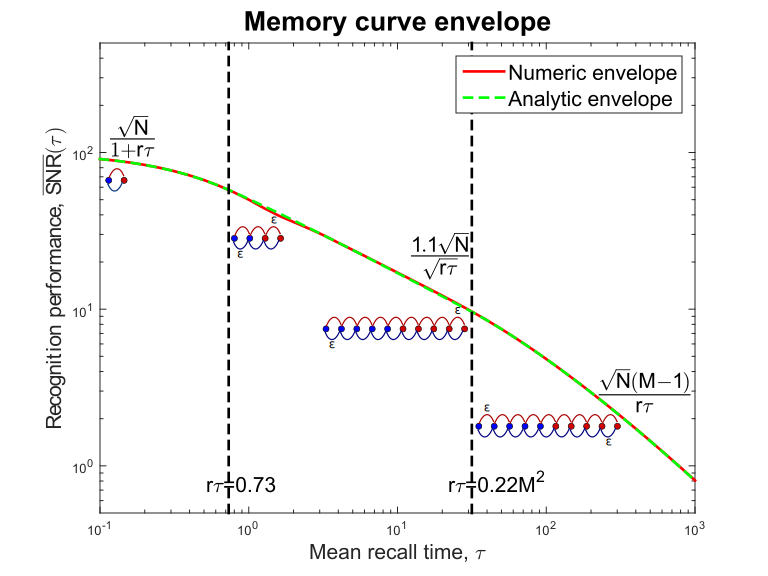
\includegraphics[width=0.8\linewidth]{LenvHeuristic.svg}\\
  \caption[Heuristic envelope]{Heuristic envelope.
  Analytic expressions are only valid to the right of each region.}\label{fig:heuristicenv}
\end{figure}



\section{Conclusions}\label{sec:conclusions}


We do not expect to find precisely these models inside real synapses.
First, evolution was faced with stronger constraints than us when designing these synapses as it had to build them out of real molecules.
Second, the set of priorities faced by evolution would have been longer than just performance in recognition memory at a single timescale.

Nevertheless, the qualitative message of our findings should be more robust to reality:
%
\begin{itemize}
  \item \emph{Short} timescale $\to$ \emph{intermediate} timescales: transition topology goes from \\ short and wide $\to$ long and thin.
  \item \emph{Intermediate} timescale $\to$ \emph{long} timescales: transition probabilities go from \\ strong and deterministic $\to$ weak and stochastic.
\end{itemize}
%
This is what we expect to find in the different brain regions that store memories for different timescales.

The transition between the two regimes is set by the maximum number of states, $M$ (we can't set the number of states to be exactly $M$, as bigger models can always mimic smaller models).
So, if we want to lengthen the timescale at which a synapse is optimal, we start by adding extra states, using the topology mechanism.
When we run out of states, we switch to the stochasticity mechanism and make the end states sticky.
The stochasticity mechanism is only used when we no longer have the option of using the topology mechanism.
It is always better to add more states, if allowed, than to make transitions stochastic.

We can get some insight into why this is by considering a serial model with $M$ states and all transition topologies equal to $q$.
%
\begin{equation*}
\begin{aligned}
  \snr(0) &\propto q,
  &\qquad
  \max_a \tau_a &\propto \frac{1}{q}, \\
  \snr(0) &\propto \frac{1}{M},
  &\qquad
  \max_a \tau_a &\propto M^2. \\
\end{aligned}
\end{equation*}
%
The initial SNR scales as described because it is related to the equilibrium probability flux between the weak and strong states, and the equilibrium distribution is uniform over $M$ states.
The lifetime scales as described because $rq$ sets the timescale for transitions, and for diffusion distance ($M$) scales as the square root of time.

If we want to lengthen the lifetime with a fixed hit on initial SNR, we get a larger increase by increasing $M$ than by decreasing $q$.
If we want to lengthen the lifetime by a fixed amount, we take a smaller hit on initial SNR by increasing $M$ than by decreasing $q$.
Thus, we always get more bang for our buck using the topology mechanism than the stochasticity mechanism.


%\subsection*{Acknowledgements}



%%%%%%%%%%%%%%%%%%%%%%%%%%%%%%%%%%%%%%%%%%%%%%%%%%%%%%%%%%%%%%%%%%%%%%%%%%
%\subsection*{Appendices}
%\appendix
%%%%%%%%%%%%%%%%%%%%%%%%%%%%%%%%%%%%%%%%%%%%%%%%%%%%%%%%%%%%%%%%%%%%%%%%%%





%%%%%%%%%%%%%%%%%%%%%%%%%%%%%%%%%%%%%%%%%%%%%%%%%%%%%%%%%%%%%%%%%%%%%%%%%%

\bibliographystyle{utcaps_sl}
\bibliography{maths,neuro,markov}

\end{document}
